\documentclass[a4paper, 12pt, twoside]{book}
\usepackage[utf8]{inputenc}
\usepackage[T1]{fontenc}
\usepackage[spanish]{babel}
\usepackage{lipsum}
\usepackage{hyperref}
\usepackage[margin=1in]{geometry}
\usepackage{graphicx}
\usepackage{wrapfig}
\usepackage{xcolor}
\usepackage{mdframed}
\usepackage[nottoc]{tocbibind}
%quotes and "fancy chapters":
\usepackage{quotchap}
%"inline" quotes
\usepackage{csquotes}
%"dialogue"
\usepackage{dialogue}
%licencia:
\usepackage[
        type={CC},
        modifier={zero},
        version={3.0}
]{doclicense}
\usepackage{verbatim}
%custom header:
\usepackage{fancyhdr}
\usepackage{float}
\pagestyle{fancy}
\fancyhf{}
\fancyhead[CE]{\rightmark}
\fancyhead[CO]{\leftmark}
\rfoot{page \thepage}


\title{Ejemplo de titulo}
\author{Yo}
\date{\today}

\makeatletter
\newcommand\mymaketitle{%
  \begin{titlepage}
    \null\vfil\vskip 40\p@
    \begin{center}
      {\LARGE \@title \par}
      \vskip 2.5em
      {\large \lineskip .75em \@author \par}
      \vskip 1.5em
      {\large \@date \par}
      \vskip 2.5em
        \graphicspath{  }               %modify this to include your own images
            
\includegraphics[width=0.5\textwidth]{figures/complutense.png}
    \end{center}\par
    \@thanks
    \vfil\null
  \end{titlepage}
}
\makeatother


\begin{document}
\mymaketitle
\tableofcontents
{\fontfamily{ccr}\selectfont

\chapter{Introduccion}
\section{Breve prefacio del autor}
\begin{wrapfigure}{l}{0.25\textwidth}
	\centering
	
\includegraphics[width=0.25\textwidth]{figures/mi_foto.jpeg}
	\caption{una foto de cuando era joven...}
\end{wrapfigure}

Soy un estudiante de Ingenieria informatica en la universidad complutense de madrid. Nunca he encajado demasiado bien en los grupos de gente, suelo tener opiniones distintas al resto, esto sumado a algunas complicaciones en mi vida de adolescente, me ha llevado a pasar algunas temporadas de soledad, que he disfrutado pues he podido reflexionar a cerca de muchisimos temas que ardian dentro de mi, y darme cuenta de lo que para mi es realmente importante. 
Normalmente este tipo de periodos se daba en epocas vacacionales, pero debido al fuerte confinamiento que hemos vivido en Espana y a la politica personal que estoy llevando ante la situacion sanitaria, he tenido mucho tiempo para esta tarea. Ha sido un tiempo para llevar a cabo lecturas que tenia pendientes y atender clases y discursos de importantes mentores o personas con una opinion distinta a la gente en general.
Estos factores sumados a mi fuego interno y mi necesidad de no dejar las cosas para otro dia, por que si no nunca las hago, ha surgido la idea de escribir estas paginas, mientras caminaba por el campo tranquilamente.
Solo espero que la lectura sea recibida con la mente abierta, pues lo requiere. En mi experiencia, en estos momentos de soledad en los que considero que he crecido como persona, estableciendo quien soy , hacia donde voy y por que principios me rijo, lo he podido hacer por que estaba abierto al cambio. 
\section{Marco de \LaTeX}
Estas paginas se entregaran como un ejercicio final de el curso de latex (basix) que se imparte en la universidad Complutense de Madrid. Aunque el profesor nos pidio que fuera algo creativo, a mi me ha salido hacer esto, he intentado aplicar varias de las tecnicas que vimos dentro del curso para que se ajuste a los requisitos en cuanto al formato, pero en cuanto a contenido ha quedado un ejercicio mas serio, pero sentia la necesidad de hacerlo y asi ha sido. Aun asi creo que ha quedado un formato de <<libro>> improvisado distinto a lo normal con cosas un poco random por aqui y por alli que enriquecen el ejercicio con estas tecnicas de \LaTeX \\

Comentar que el ejercicio lo he elaborado en su mayoria \textit{offline} con un editor de texto y el paquete \textit{texlive-full} de linux. El codigo esta disponible en \href{https://github.com/dlgeraghty/basix-latex/tree/master/independencia/template}{mi github} \\

Para la documentacion basicamente he utilizado las guias que proporciona overleaf \textbf{INSERTAR REFERENCIA AQUI}

\chapter{Antes de leer estas paginas}
\section{Aviso}
\begin{mdframed}[backgroundcolor=yellow]
	
\includegraphics[width=0.05\textwidth]{figures/warning.png}
	El contenido que vas a leer a continuacion puede resultar politicamente incorrecto dependiendo del lugar/epoca en la que estes leyendo esto
	
\includegraphics[width=0.05\textwidth]{figures/warning.png}
\end{mdframed}
\section{Motivacion para la lectura}
Sientes con frecuencia que tienes comportamientos diferentes segun con el grupo de personas que estes? Eres una persona a veces y otras veces otra? 
Cuando estas con gente, haces cosas que normalmente no harias para sentir que perteneces al grupo? 
Si en un grupo, los demas estan haciendo algo que no te apetece, como te sientes? 
Tienes alguna meta clara en la vida, persigues algun objetivo? Es posible que te hayas propuesto algo por influencia de los demas sin pararte a pensar si realmente es lo que quieres? 
Cuando tomas decisiones que tienes en cuenta? Te frena \textit{el que diran} cuando estas pasando por el camino hacia tus metas?
Cuando te pasa algo, como una situacion sobrevenida negativa que no te esperabas, eres capaz de reaccionar ante ella para salir mas fuerte o culpas a agentes externos?
Si alguna de las anteriores preguntas te ha chocado o te ha hecho pensar, te animo a seguir leyendo y descubrir cosas nuevas. 

Es cierto que vivimos en sociedad y que negarse a ello seria luchar contra la naturaleza, pero hay sociedades en las que los individuos no son por si mismos, solo en sociedad. Las metas que se han establecido son probablemente impuestas por los estandares de la sociedad sin pararse a reflexionar. De esta forma, en ocasiones, el motivo de su vida es esa sociedad.
Yo mismo he podido ver como gente que tenia una opinion fuerte a cerca de un tema, rompieron su integridad sin pensarlo mucho y como saben que lo que han hecho iba en contra de sus principios, buscan apoyo en la opinion de los demas que les es favorable y asi se justifican. 
\subsection{Historia que invita a la reflexion}
Esto es lo que me parece mas grave, y pondre un ejemplo, consta de dos personas, que llamaremos \textit{uno} y \textit{dos}:
(Esta historia ha sido ligeramente modificada para estresar el problema que quiero comentar)

Uno ni se planteaba en su vida fumar, era algo contra lo que tenia una opinion fuerte sustentada por si mismo. Uno se mantuvo integro un tiempo, sin embargo yo desde fuera veia que en ocasiones se dejaba llevar un poco en este tema. Ante mis avisos, lo que obtuve fueron reprimendas sociales. El dia llego en el que finalmente tiro este principio por la ventana e hizo lo que dijo que nunca haria. La justificacion fue bastante curiosa, \textit{es que dos se tenia que acabar su cajeta y le sobraban}. Y por supuesto, mientras lo seguia haciendo seguia encontrando justificaciones. Curioso cuanto menos no? 

Es a este tipo de actos, aunque el que he retratado anteriormente es meramente anecdotico y en una escala de peligro es bajo, pues como mucho se hara dano a si mismo, a los que me refiero cuando digo que las sociedades pueden resultar malas (malas en el sentido de que corrompen nuestros principios) si no se tiene la suficiente fuerza para decir no en este caso, o en otras palabras, ser verdaderamente independiente. 

Pensemos por un segundo en el ejemplo anterior que habria pasado si uno le hubiera dicho a dos que no que no lo haria, que si se los tenia que acabar los podria tirar a la papelera. Uno se habria mantenido integro a sus principios, pero que habria pensado dos? Quizas habria sentido rechazo al ver que uno no cederia, esto en ocasiones en mi experiencia deja ver cierta inseguridad en dos, pues una de sus formas de justificar lo que hace es que lo demas lo hagan, es algo como: \textit{o estas conmigo o estas contra mi} y eso crea una presion fuerte en las relaciones entre personas especialmente en grupo cuando hay \textit{"1 contra N"} 
 
\subsection{Por que independencia?}
Mi definicion de independencia:
La independencia es libertad para actuar acorde con los principios que hemos desarrollado por nosotros mismos, que no tienen que ser fijos ni estaticos durante toda la vida, pero tienen que venir de forma genuina de nosotros. Cuando tenemos esta libertad y somos integros con nuestros principios, estaremos completos por nosotros mismos y no necesitaremos de los demas para justificarnos. Las relaciones interpersonales toman otro rumbo mucho mas enriquecedor y puro pues nosotros ahora sabemos lo que queremos y podemos ver los puntos de vista de los demas como una experiencia diferente y enriquecedora y no como algo que tenemos que adoptar para ser parte del grupo.
Como hemos visto en la historia anterior, es necesario tener principios claros y muy importante tambien es ser lo suficientemente fuerte para aguantar la presion social y saber decir que no en ese caso, pero la independencia noes solo en lo social, hay otros ambitos importantes.
\subsection{Cual es el minimo grado de independencia?}
Como ya comentaba, y ahora sintetizo, creo que el minimo grado de independencia que uno debe tener es el suficiente para actuar en contra si es necesario de la sociedad o los grupos que le rodean si asi cree en ello. No hacer lo que hacen los demas, la imagen mas clara es la del rebano de las ovejas que no saben hacer otra cosa que seguirse las unas a las otras en contraste con el lobo que se vale por si mismo cuando esta solo pero \underline{cuando va con la manada se crece y multiplica sus fuerzas}, esto es, es \textbf{interdependiente}
\subsection{Por que la independencia no es suficiente?}
Como comentaba en el punto anterior con el lobo que es perfectamente capaz de valerse por si mismo sin necesitar de los demas, no sigue al rebano de ovejas, pero como es independiente por si mismo, cuando se junta en manada con otros lobos independientes, juntos son capaces de hacer cosas increibles.
Esto es el paso siguiente a la independencia

\subsection{Mis influencias}
En la introduccion comentaba que cuando estas abierto al cambio es cuando realmente tienes la capacidad de aprender y crecer como persona, y que para ello lo mejor que puedes hacer es leer, atender clases de profesores y rodearte de gente que te enriquece. Esto es muy dificil pues mucha gente tiene segundas intenciones y puede tratar de manipular, sin embargo yo creo que encontre muy buenos apoyos en las siguientes fuentes:
\begin{itemize}
	\item{ \textit{the 7 habits of highly effective people} de Stephen R Covey 
		\begin{figure}[h]
			\centering
			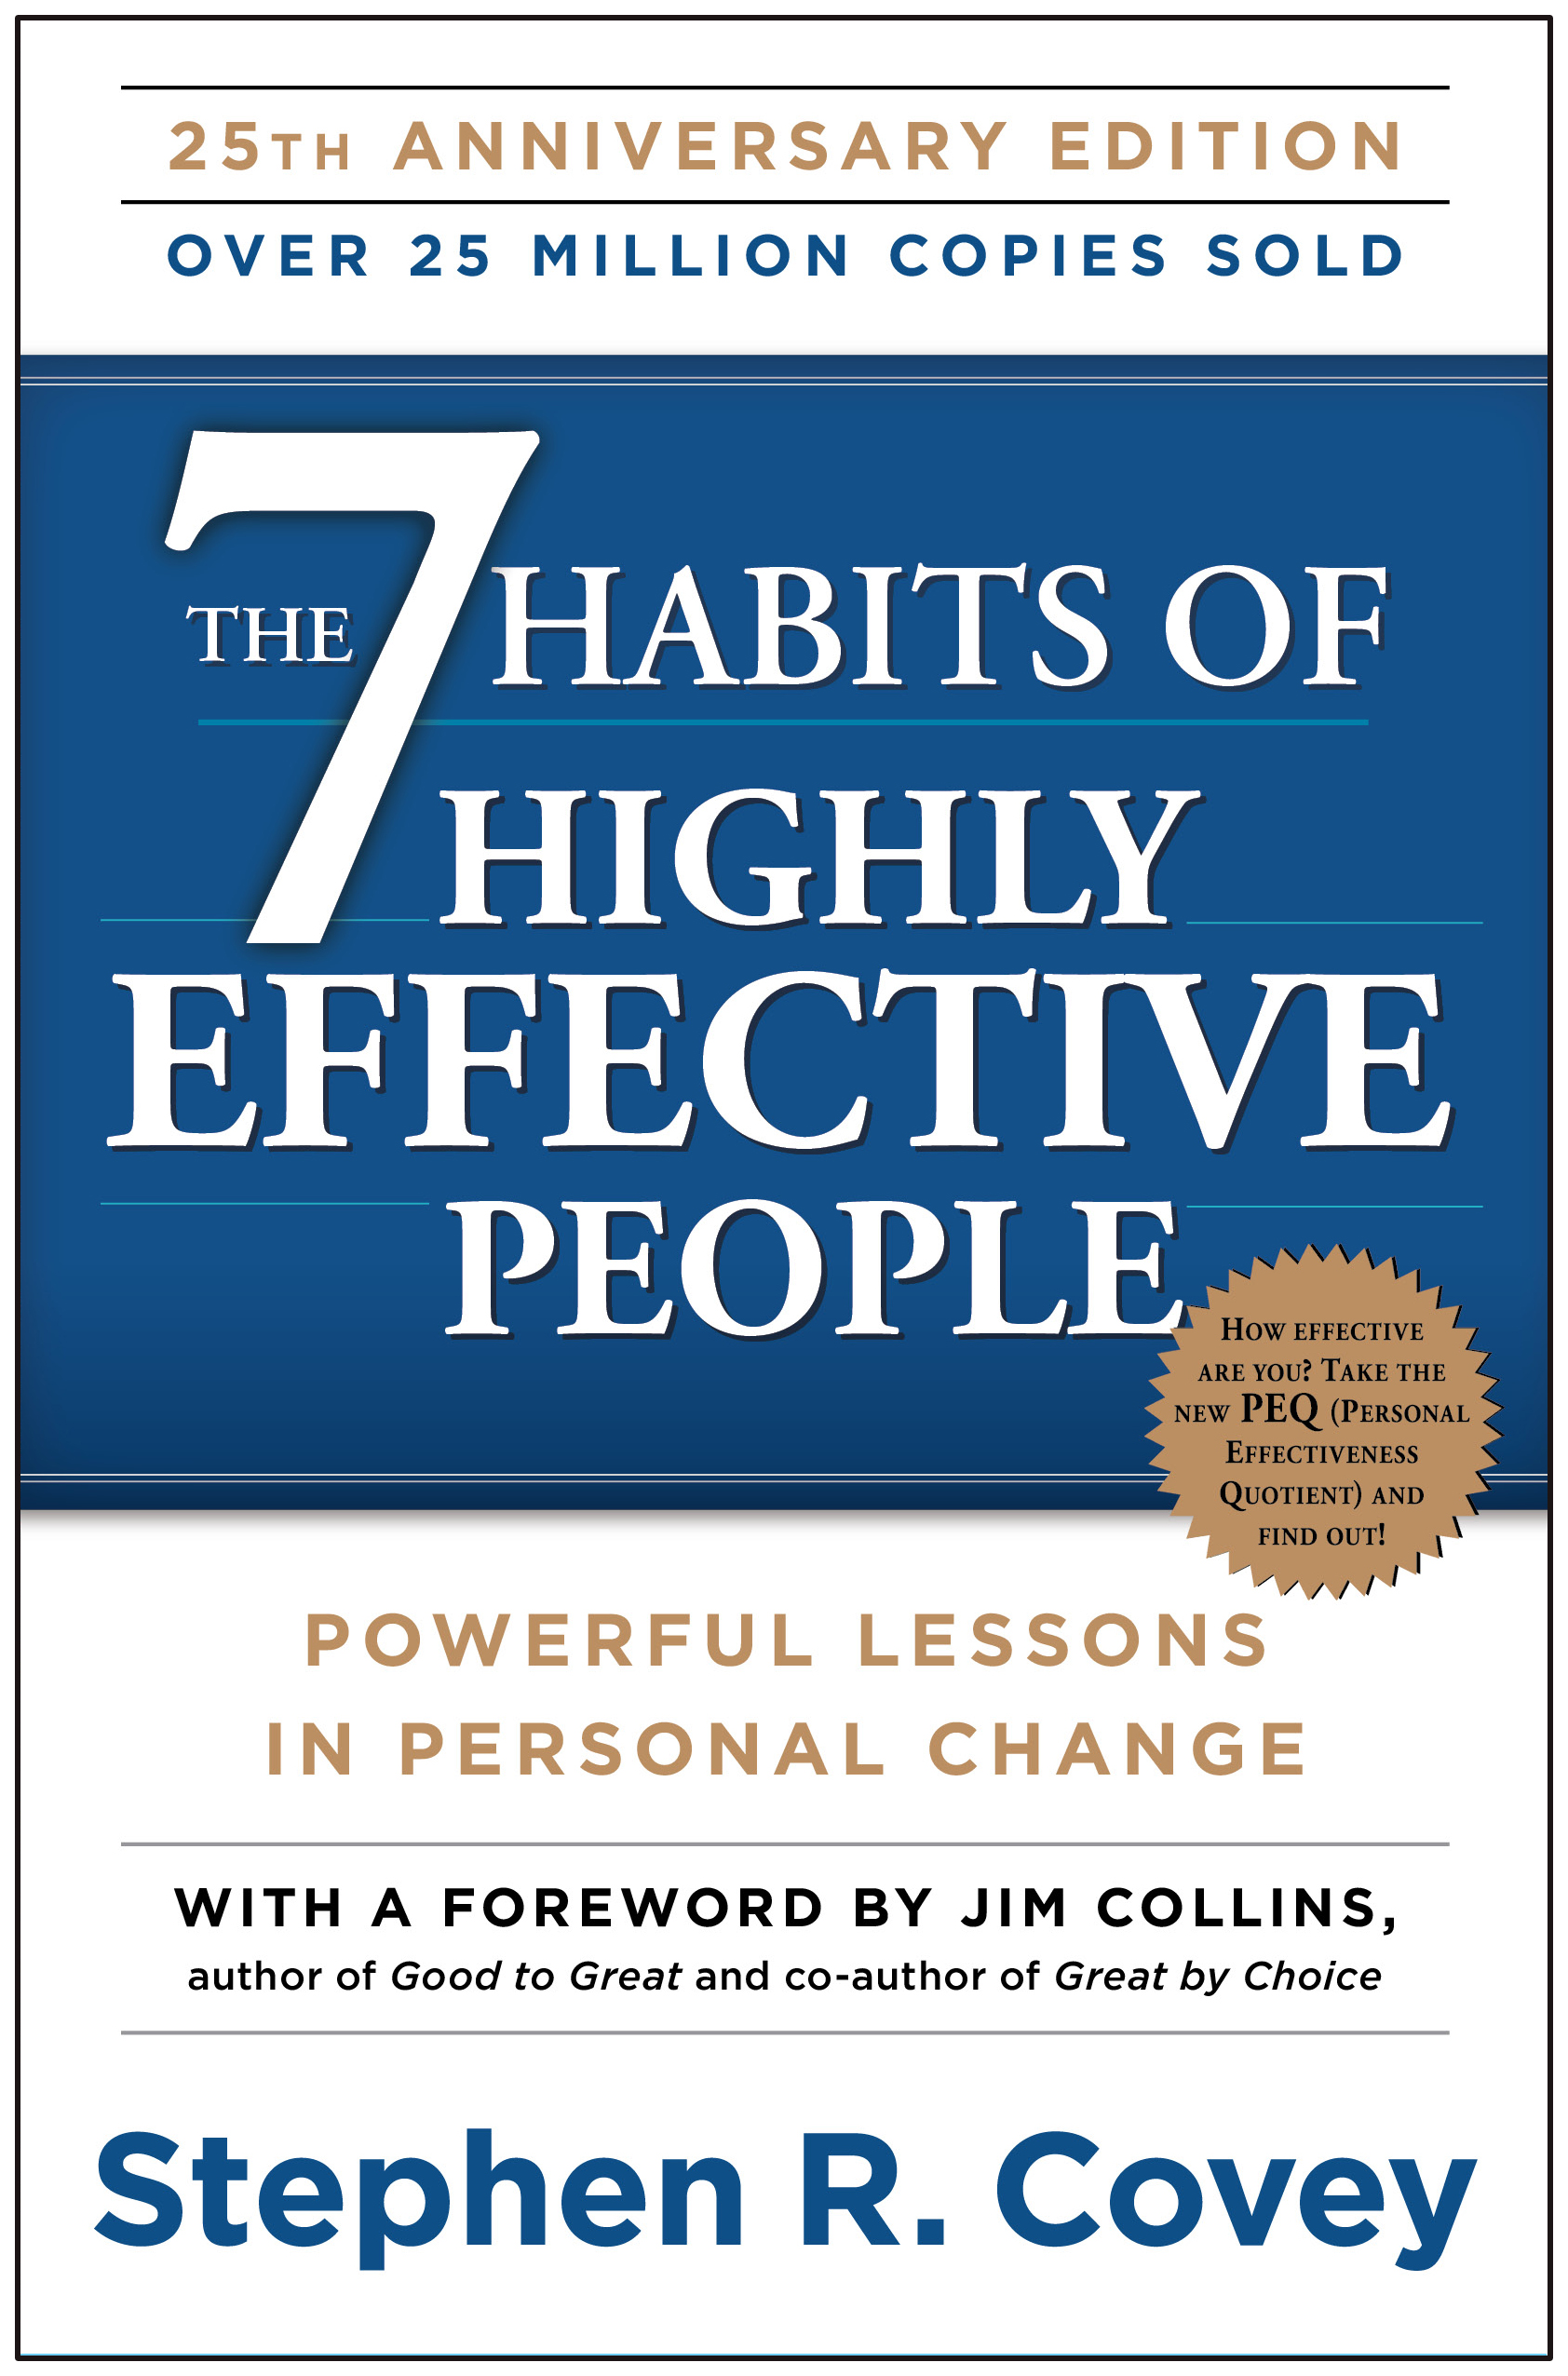
\includegraphics[width=0.4\textwidth]{figures/the7habits.jpg}
			\caption{The 7 habits of highly effective people by Stephen R Covey}
		\end{figure}
	}
\item{ canales de youtube que hablan sobre independencia en el ambito de la informatica: luke smith o distro tube
		\begin{figure}[H]
			\centering
			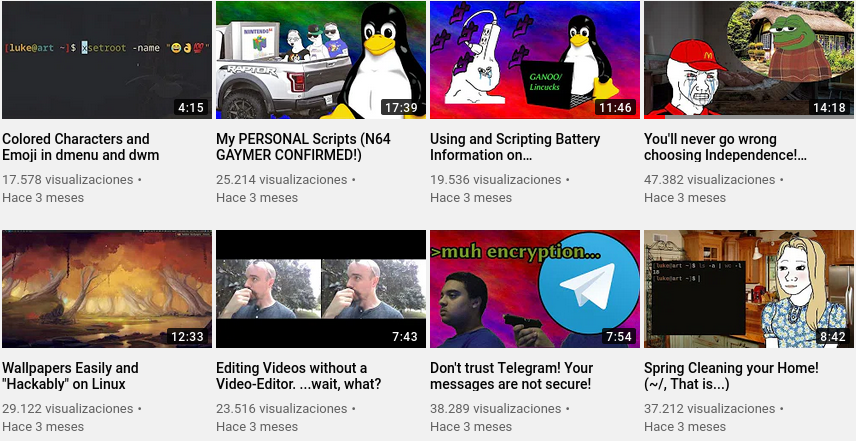
\includegraphics[width=0.75\textwidth]{figures/luke-smith.png}
			\caption{Captura de pantalla de las portadas de algunos videos de luke smith}
		\end{figure}
	}
	\item profesores como juan ramon rallo que apelan a la reflexion sobre las decisiones politicas en nuestro pais dando un punto de vista lleno de datos objetivos (fundamentalmente aboga por la libertad en la economia)
\end{itemize}

Estas fuentes no han hecho mas que poner en forma de palabras y ampliar conceptos en los que yo ya creia, es por eso que creo que han sido tan enriquecedoras. No es que lo haya leido y me haya convertido en defensor de la independencia, si no que ya creia y actuaba de forma indpeendiente y luego me tope con estas fuentes que me enriquecieron pues era gente mas sabia que ya habia vivido mucho mas que yo y que me confirmo que no solo es posible recorrer este camino si no que en sus palabras los resultados son maravillosos. Yo creo por tanto que es sabio aprender de gente que tiene los resultados que nosotros queremos alcanzar.

He de citar tambien una pelicula que me parecio increible en este aspecto pues era una historia de superacion distinta a las demas, no solo el personaje sufria un accidente y era capaz de recuperarse para los juegos olimipicos, si no que el cambio fisico positivo le vino por una voz interior que le enseno a ser independiente, se llamaba el camino del gerrero.


\chapter{Como saber quien eres}
\section{dos herramientas}
Esto es algo curioso y un tema muy profundo, yo solo te dare dos herramientas que creo que te pueden ayudar mucho en la busqueda dentro de ti para saber que valores te definen.
\begin{enumerate}
	\item El dia de tu funeral, que tres cosas te gustaria que dijeran de ti
	\item Experimenta todo lo que puedas en tu vida acorde a tus valores
\end{enumerate}

\chapter{El Habito}
\section{ Que es el habito }
Mi entendimiento de habito es una accion que repetimos en el tiempo \cite{lally2010habits} de tal forma que la hacemos nuestra en el sentido de que pasa a formar parte de nuestras actividades \underline{normales} y nos puede llegar a resultar fisica o psicologicamente dificil dejar de practicarlo. 
\section{ Que tiene que ver con la (in)dependencia?}
Que pasa cuando llega el verano y como estudiantes no tenemos que trabajar y por tanto nos podemos relajar y dormirmos a las tantas de la noche y levantarnos casi a la hora de comer?

Creamos ese habito y lo asociamos con sentimientos positivos como la felicidad, comodidad, descanso...etc. Esto es lo que en ocasiones provoca que cuando comienza el curso y yo este en la parada del autobus esperando para ir a la universidad, oiga comentarios como \textit{"que pereza"}, o \textit{"que conazo"}. Aqui hay un gran problema que es mas grave de lo que pueda parecer en un primer momento, y es que no solo hemos creado un habito que ya de por si podria resultarnos complicado o costoso renunciar a ello si no que lo hemos asociado a unos sentimientos positivos por lo que si tenemos la necesidad de romper este habito podriamos asociarlo a sentimientos negativos. 

Esto puede parecer una tonteria pero algo tan simple como levantarnos cada dia, si lo asociamos con sentimientos negativos (por que tenemos cierta dependencia de levantarnos mas tarde) puede ser la diferencia entre un dia productivo o miserable, y esto se puede extender en el tiempo.

Lo que quiero decir con esto no es que nos levantemos todos los dias a las 5 de la manana para aprovechar el dia y asi ser mas productivos. En epocas vacacionales yo personalmente y mcha otra gente recomienda descansar y disfrutar, ademas si gozamos del privilegio de no tener que trabajar o tener un horario muy flexible podemos aprovechar a dormir mas o ir a la cama mas tarde. Lo que yo vengo a reivindicar aqui realmente es que tenemos que ser conscientes de que cuando terminen las vacaciones y volvamos por ejemplo a clase es posible que nos tengamos que levantar a las 6 o 7.

\textit{Un gran poder conlleva una gran responsabilidad} y en este caso, el gran poder que tenemos es el de no tener que ajustarnos a un horario fijo (en un sistema en el que fueramos financieramente independientes quizas podriamos gozar de esto tambien) pero la responsabilidad es que llegado un punto tendremos que volver a hacerlo y tenemos que tener la fuerza interna, mental, suficiente para poder llevar a cabo esta accion.

El hecho de decir, vale, soy consciente de que estoy en un periodo vacacional y tengo menos obligaciones, ademas por mi situacion personal en los distintos ambitos fundamentales (salud, economia y relaciones) puedo permitirme relajarme durante este tiempo, pero soy perfectamente consciente de que no puedo establecer esto como mi normalidad a partir de ahora.

Si cometemos el error de establecer un habito como este como nuestra normalidad, cuando sabemos de antemano que por nuestras circunstacias ese habito solo lo podremos llevar a cabo durante un tiempo determinado (ej. 2 meses de verano) y luego tendremos que abandonarlo, estamos cometiendo un grave error. 

Mi consejo ante esta pequena anecdota es que disfrutemos de estos pequenos privilegios o lujos que podemos darnos pero no lo establezcamos como lo normal, que seamos conscientes de que dentro de un tiempo tendremos que dejar de hacer esto y que antes de permitirnos este lujo, evaluemos si somos suficientemente fuertes como para dejarlo.

Hay veces que creemos que somos fuertes para dejarlo y por tanto nos damos la licencia de permitirnos un lujo, pero a medida que va avanzando el tiempo y nos acostumbramos a ese lujo, la fuerza que teniamos o creiamos que teniamos al principio se va desvaneciendo.

Yo creo que cada uno nos tenemos que ganar los lujos por nosotros mismos, habiendo pasado por ganar la fuerza necesaria que corresponde con lo contrario a ese lujo. Asi, yo creo que en nuestro ejemplo anterior, si nos hemos levatado durante el curso a las 6 todos los dias religiosamente, \textbf{POR CONVICCION INTERNA NUESTRA Y NO POR IMPOSICION}, probablemente hayamos "ahorrado" la fuerza suficiente para poder permitirnos el lujo de dormir hasta tarde pero luego ser capaces de rapidamente "romper esa hucha" donde teniamos depositados los ahorros correspondientes a la fuerza para levantarnos temprano y asi adaptarnos a nuestra nueva realidad.

Es importante resaltar que he dicho que ahorramos fuerza durante un periodo en el que realizamos un habito de forma independiente, luego durante otra temporada nos damos el lujo de romper con el primer habito creando un segundo habito que es contrario al primero. Es importante decir que pasar de desperarse pronto a despertarse tarde es algo que no requiere mucha fuerza de voluntad o no requiere que "gastemos los ahorros de fuerza", al menos asi lo creo yo para la mayor parte de gente normal. Pero que pasa cuando tenemos que pasar de despertarnos tarde a desperatarnos temprano? Logicamente esto cuesta mas, requiere un esfuerzo adicional pues hemos estado tan comodos y hemos asociado sentimientos positivos a despertarnos tarde de tal forma que necesitamos "un empujon" para ir en contra de esos sentimientos positivos y de esa comodidad. 

Me gustaria hacer un inciso por que sin ser un profesional en esto veo que hay un cierto comportamiento que es mas comun de lo que parece, y es que cuando tenemos que romper con un habito positivo y comodo para nosotros hay gente que lo toma con una motivacion externa y esto lo considero un error. Me explico, por ejemplo para comenzar a ir a clase, y por tanto romper con los habitos que habiamos adoptado durante las vacaciones, podriamos coger motivacion externa de amigos que tambien van a clase y por tanto nos motivan a ir o de actividades que se realizan al comienzo de las clases para motivar a los estudiantes. Esto para mi es un error importante por que si no tenemos ahorros propios de fuerza interna para hacer algo si no que \textbf{dependemos} de los demas o de fuentes externas para que nos motiven a hacerlo, que pasara el dia que esas fuentes no esten? o si cambian las campanas y ya no nos motivan? El resultado de esto sera, en general, que no encontramos la motivacion para hacer las cosas. Por eso creo que el hecho de \textbf{depender} de fuentes externas para motivarnos es \textit{pan para hoy, hambre para manana}, poner tiritas en una herida profunda que requiere una operacion.

Esto viene a que debemos tener esos depositos de fuerza interna que sean en la medida de lo posible \textbf{independientes} de fuentes externas y por tanto cuando tengamos que levantarnos temprano y sintamos esa resistencia inicial, podamos echar mano de los ahorros de fuerza, que no es mas que la motivacion interna que tenemos para hacer algo. 

Todo esto anterior presuponia que sabemos que algo contrario a lo que nosotros nos hemos permitido como lujo va a ocurrir, pero que sucede cuando no sabemos de antemano que eso va a pasar? 

Este tipo de situaciones son lo que puede marcar la diferencia, ya que nosotros nos acostumbramos a un cierto estilo de vida a unos habitos que \textbf{dependen} de factores que aun siendo externos a nosotros, tenemos la conviccion interna de que esos factores no nos van a fallar, que siempre van a estar ahi cuando los necesitemos y la realidad es que no.

Hare un simil con un tema que probablemente pueda ser polemico pero es que a mi me parece que la gestion de las emociones de una persona es similar a la gestion economica, yo creo que al igual que en economia si queremos ser minimamente independientes debemos ahorrar dinero para cuando pueda venir una crisis, en la gestion de nuestras emociones debemos ahorrar en una forma menos tangible, deberiamos trabajar en nostros mismos cada dia un poco al igual que lo hacemos por dinero, por nosotros. Asi cuando venga una crisis emocional provocada por una situacion negativa podremos paliarla mejor.

Como podemos trabajar en nosotros mismos? Te estaras preguntando, pues es realmente sencillo para mi, yo creo que tenemos que hacer pequenas acciones que nos permitan definir quienes somos y seguir nuestro camino. Para acometer esto, nada mejor que tener muchas experiencias de gente sabia que ya recorrio el camino, por que al igual que en las finanzas es siempre mas conveniente aprender \textit{con el dinero de otros}, esto es, por sus experiencias y operaciones, yo creo que en el ambito sentimental y de la vida tambien se puede hacer esto.

Una de las formas que yo encuentro personalmente mas fascinante es escuchar historias de gente que estaba en situaciones malas y que salio adelante con mucha fuerza, asi me entreno en parte, sabiendo que por muy duro que sea lo que estoy pasando, puedo salir adelante y ademas salir reforzado. Esto lo he hecho durante muucho muucho tiempo, uno de los mejores medios es el canal de youtube de Fearless Motivation y similares.

Estas historias me han preparado para tratar situaciones muy dificiles que han terminado ocurriendo en mi vida, pero tambien el entrenamiento fisico es una de las actividades que a mi independientemente de todo lo demas me ha ayudado a salir adelante.

Puedo firmemente aconsejar estos medios para lograr ser una persona mas entrenada ante situaciones dificiles y saber salir de ellas de la mejor forma posible, incluso reforzados. 
\section{ Crear/cambiar habitos}

Como vemos esto de los habitos no es ninguna tonteria, un mal habito es como una mala inversion, y si lo asociamos a sentimientos muy positivos de forma que es muy dificil deshacernos de ello es como aplicar mucho apalancamiento en una operacion y que nos salga mal, nos podemos quedar estancados o irnos a la bancarrota.

Irse a la bancarrota en las finanzas o economia puede ser un golpe durisimo en nuestra vida, pero irse a la bancarrota internamente como personas, desarrollar y mantener habitos toxicos para nosotros mismos buscando el apoyo de los demas o el reconocimiento de factores externos puede determinar nuestra vida de una forma mas drastica de lo que la gente reconoce. 

Yo soy partidario como decia anteriormente de escuchar historias de las vidas de otras personas, especialmente de aquellos que son exitosos y a los que nos queremos parecer, y ver si forma de vida y habitos es, salvando las distancias, comparable a la nuestra y en que medida. Siempre podemos aprender algo y lo mejor, escuchar la historia de otras personas nos puede hacer reflexionar y llegar a la conclusion de que un habito de los que estabamos llevando a cabo podria ser un elemento contraproducente en el camino a completar nuestras metas.

Pero ojo y mucho cuidado, esto puede ser tanto positivo como negativo, por tanto yo creo que es determinante antes de "dejarnos influenciar" o tomar nota de lo que hacen otras personas deberiamos tener claro al menos cual es el camino que queremos seguir en cierta medida, no hace falta que hayamos trazado cada instante de nuestros proximos anos de vida y que lo sigamos a rajatabla, pero si que sepamos al menos el camino hacia el que queremos ir, que lo hayamos meditado y que creamos muy fuerte en nosotros mismos. Digo esto por que igual que yo me puedo plantar por ejemplo a ver un video de Steve Jobs, un documental sobre su vida por ejemplo, y captar como ideas positivas la forma en la que el creia en si mismo y lo claras que tenia las cosas, la vision que tenia y lo innovador que era para su tiempo, alguien puede ver esta historia desde otro punto de vista o le pueden contar otras partes y sacar como conclusiones que las drogas son positivas para tener ideas, que para poder perseguir tus suenos tienes que dejar la universidad, que acostarse con una persona y luego dejarla tirada incluso cuando tiene un hijo tuyo renegarlo...esto a mi personalmente no me representa segun mis valores.

Lo que quiero decir con esto es que cuidado, volviendo a nuestra historia del principio de fumar, existe el famoso argumento de \textit{pero si te vas a morir igual} que he escuchado muchas veces, y otro tipo de argumentos de este tipo que son mas bien creencias populares y que en ocasiones no estan bien fundamentados mas que en la opinion popular...pues resulta que este tipo de argumentos al menos en mi experiencia resultan muy cautivadores por el hecho de que es la creencia popular, es lo que la mayoria de personas piensa y por tanto pueden llegar a ser persuasivos. Es en estos momentos donde tenemos que plantearnos si este tipo de actos nos van a ayudar a avanzar en nuestro camino hacia nuestras metas y suenos o por el contrario nos van a hacer retroceder.

Hay un dicho en el mundo de la bolsa, que dice \textit{esto es 90\% psicologia y 10\% conocimiento}, pues yo creo que muchas de las situaciones de la vida, las decisiones que tomamos, se ven mucho mas influenciadas por la psicologia interna que por el conocimiento que tenemos.

Es por esto que yo considero fundamental tener una psicologia muy fuerte y que hayamos creado nosotros mismos.

Pero bueno, que nos desviamos del tema, esto simplemente eran unas notas que queria incluir sobre como adoptar nuevas ideas de habitos.

Yo recomiendo aprender una nueva cosa cada dia, un dia yo me puse a hacer ejercicio fisico y vi que no era malo en ello y he seguido el camino hasta un punto en el que llevo mucho tiempo en que el ejercicio fisico es un habito. Otro dia me sentia inspirado para tocar el piano y al ver que la curva de aprendizaje requeria mucho mas sacrificio del que yo estaba dispuesto a hacer, no me lo he tomado tan en serio, no es algo a lo que yo este dispuesto a dedicar el mismo esfuerzo que al entrenamiento fisico y eso no significa otra cosa que no lo quiero tanto. Un dia considere poner a prueba mi habilidad para montarme un ordenador de la forma mas barata posible, llevaba ya tiempo preparandome mentalmente para ello, habia creado ese habito, pero eso solo era la teoria, ahora me iba a probar a mi mismo en la parte practica.

Lo que quiero decir con esto es que es muy bueno probar cosas nuevas, por supuesto no todos los dias nos podemos plantear montar un pc, pero si que nos podemos plantear meternos en internet y buscar informacion sobre ello, estimar la cantidad de esfuerzo que requiere y decidir si nos merece la pena o no o si estamos dispuestos a hacerlo.

Me parece extraordinariamente importante recalcar que esta curiosidad por investigar nuevos temas ha de salir d e nosotros mismos, no de los demas, por ejemplo el gimnasio creo que es el area donde esto se ve mas claramente. A menudo vemos que hay gente que trata de ponerse en forma, se ponen unos objetivos y se apuntan a un gimnasio, pero en algunas ocasiones no lo estan haciendo por ellos mismos, si no por los demas: \textit{oye, tu tienes que ponerte en forma e} o \textit{despues de vacaciones nos apuntamos} pero solo lo hacen por la opinion que los demas tienen de ellos. Yo por ejemplo sin embargo comence a hacer ejercicio en mi casa tranquilamente, sin darle demasiada importancia, y asi segui y segui hasta que un dia me atrevi a ir a un parque de barras donde habia mas gente, pero como yo ya tenia el habito no me afectaba a niveles fundamentales la opinion que los demas tenian de mi, yo sabia quien era y lo que me habia costado llegar hasta ahi.

Lo que quiero decir con esto, es que los habitos mas potentes son aquellos que desarrollamos de forma independiente por curiosidad de descubrir una faceta de nosotros que nos gustaria explorar. En mi opinion los habitos que nos vienen impuestos por otras personas directamente o indirectamente por la opinion de la sociedad, no solo son debiles si no que pueden llegar al punto de debilitarnos a nosotros por que puede no gustarnos lo que hacemos y a partir de ahi podemos llegar a plantearnos cuestiones mas fundamentales sobre nuestro ser que nos pueden llevar a conclusiones muy buenas pero tambien a conclusiones muy negativas.

Abandonar un habito que tenemos puede llegar a ser complicado, pero mi mejor consejo para ello es quedarnos impactados ante la forma de vida que tienen otras personas a las que admiramos y que quizas no cuentan con ese habito, lo cual nos puede llevar a plantearnos si es realmente necesario para nosotros. Pero tambien es muy importante como comentaba anteriormente intentar minimizar el numero de habitos que tenemos que han sido impuestos por los demas, pues estos levantaran ,probablemente, dentro de nosotros sentimientos negativos. Si nos encontramos en la situacion de que ya estamos llevando a cabo habitos impuestos que no nos hacen sentir bien o nos hacen sentir mal, lo mejor que podemos hacer es buscar la manera de renunciar a ello para hacer algo con lo que nosotros mismos nos sintamos llenos y productivos.


\chapter{La independencia}
\section{Como alcanzar la independencia}
Si has llegado hasta este punto probablemente te estes planteando esta cuestion. Y es que es cierto que no es algo trivial, yo \textbf{nunca te dare \textit{la solucion}, si no herramientas que considero te ayudaran a construir tu propia solucion}.\\

Esto para mi es una clave de la vida y no es que me desvie del tema, por que la \textbf{proactividad es un punto clave} si queremos ser independientes, si nos ponemos como meta la independencia tenemos que tener claro que tendremos que hacer mucho mucho trabajo que a lo mejor no es reconocido instantaneamente, pero ten por seguro que si has trabajado duro de forma honesta acorde a tus valores, los beneficios vendran por si solos.\\

Esto esta bien, es lo que hace la mayoria de la gente, mirar a hoy, al dia despues, a dentro de un rato, a una semana, a un mes...otro punto clave de la independencia considero que es \textbf{tener una vision de futuro clara} o al menos un camino, como comentaba en otro capitulo no lo tienes que tener todo clarisimo y fijo, pero si que conviene que definas tu camino al menos. Esta vision es lo que te va a ayudar a empujarte hacia ella y a hacer trabajo sin recompensas inmediatas, pues sabes que estas trabajando duro por algo mas alla de lo tangible, por un sentimiento, por una meta. Y diras, pero eso no me va a pagar las facturas, y yo te puedo decir que seguro que si lo hara, aunque te veas en la situacion de tener pocas posesiones materiales o problemas con el dinero, analizalo, pero si de verdad crees en tu vision, el dia llegara en que seras recompensado. Cuantas personas famososas incluso de la lista forbes no perdieron todo antes de llegar a donde estan o empezaron sin nada. Quiero hacer un pequeno apunte y es que cuando digo que definamos nuestro camino esto no es algo estatico, lo bonito de hecho es que mientras que lo vayamos recorriendo, probablemente lo iremos modificando poco a poco.\\

Intentare reflejar este conocimiento teorico con algunas anecdotas que relato a continuacion: En mi universidad un dia estaba hablando con una persona, me dijo que nunca podria llegar alto dentro de una empresa y mucho menos por mi mismo si no era por enchufe. Me parecio bastante curioso y se me quedo marcado, aunque yo creo que elijo mi propio destino y que puedo llegar a donde me proponga pero bueno. El caso es que en uno de los podcast de Fearless Motivation estaban comentando como gente que nace pobre se puede volver rica en terminos economicos por ejemplo, pero tambien en otros terminos como sociales, intelectuales...pero la parte importante venia cuando decian \textit{los padres ricos que nacieron en familias humildes les dan a sus hijos todo, todo menos las condiciones que les llevaron a ellos a ser ricos} a mi forma de ver con esto quieren decir que estos padres cuando eran ninos o adolescentes, sintieron una necesidad de trabajar mas, decidieron perseguir sus suenos y encontraron la manera, que ademas suele ser mas ingeniosa y sufrida en estos casos, de hacerlo sin el apoyo inmediato de sus familiares por que no tenian la capacidad economica para arrancar su empresa por ejemplo. Asi, ante la falta de algo como es el dinero, y el planteamiento de una meta o un sueno, consiguieron ese dinero, y ahora con el pagan todos los suenos de sus hijos que no se veran motivados a encontrar otra manera o trabajar duro por que con pedir el dinero a los padres lo pueden tener todo **(en algunos casos, notese que yo no tengo nada en contra de los padres ricos que se permiten lujos, es solo para exagerar el ejemplo).\\

Esta historia me parece paradojica pero curiosa, a parte me veo en la obligacion moral de comentar el techo que te estas poniendo a ti mismo si te levantas cada manana pensando que no puedes llegar mas alto que x posicion o no puedes llegar a tener mas de x dinero por el mero sitio en el que naciste. Es muy peligroso este sentimiento pero muy facil acoplarse a el pues asi puedes culpar a algo como el sistema de todas tus penurias (te justificas) lo cual es infinitamente mas sencillo que plantarte de cara al mundo y decir yo lo voy a conseguir, voy a trabajar duro y voy a hacer todo lo que este en mi mano por conseguir este sueno, voy a hacer sacrificios, no ire de fiesta, vivire con una politica economica de auesteridad y ahorro, no voy a caer en el consumismo o en otras trampas que me envuelven en una espiral de negatividad, voy a ser verdaderamente responsable y consecuente con mis acciones, si fracaso lo aceptare, aprendere la leccion y comenzare de nuevo pues ahora soy mas sabio y estoy un paso mas cerca de conseguir lo que me he propuesto, nada ni nadie tiene la fuerza psicologica para pararme los pies.



\section{Independencia en la toma de decisiones}
Ahora hablare de otro punto que considero fundamental, como te digo, todo esto son pequenas ideas para que mejores o evalues tu \textit{mindset}. \textbf{Tu eres el unico que toma tus decisiones}, si sientes que es la sociedad en general o un grupo de gente quien toma las decisiones por ti, probablemente estes dentro de una relacion de dependencia. Con esto no te digo que te vuelvas radical de la noche a la manana y digas que te vas a vivir solo, que te vas del trabajo, etc...\textit{(aunque esto puede puede llegar a ser algo positivo en algunos casos, no querria que se entendiera esa idea y no es un consejo que daria a alguien menos si no le conozco)}, lo que te digo es que evalues y que seas consciente de que aunque tu creas que haya cosas que tienes que hacer si o si por que otros te lo han dicho o "por que si", por que asi he nacido, por prejuicios sociales, etc...En ultima instancia tenemos que reconocer que los que tomamos las decisiones somos cada uno de nosotros, aunque esas decisiones sean seguir al rebano. \\

En este ambito, nos tenemos que hacer fuertes, tenemos que comenzar a evaluar las areas en las que estamos siendo dependientes y comenzar a darnos cuenta de que las decisiones que tomamos no estan fundamentadas en ningun criterio que hayamos desarrollado nosotros. Hay que evaluar cada una de estas areas e ir haciendo cambios poco a poco, atreverte a decir no, a preguntar lo que nadie se atreve a preguntar, a cuestionar a los demas siempre con respeto, a plantear ideas que parezcan muy locas y que todo el mundo nos llame locos, que digan que no podemos conseguirlo. Con esto te animo a experimentar diferentes alternativas que te ayuden a recorrer tu camino, ver cual se adapta mejor, pero por favor, se consciente de que \textbf{tu has llegado hasta el sitio donde estas en la vida por tus propias decisiones, y si lo decides puedes cambiar las decisiones que vas a tomar y por tanto cambiar de sitio en la vida}, esto es lo que me parece fundamental, que nada ni nadie te pare.\\

Algo que me parece bastante curioso y me parece una de los efectos mas fascinantes de la vida es como tomamos decisiones en el momento presente, y que luego al evaluarlas desde un momento futuro nos damos cuenta de que podriamos haber tomado otras decisiones mejores. Esto me parece magia, pero a la vez fundamental, y es que repasar algunos eventos en los que tuvimos que decidirnos entre varias alternativas yo lo veo una cosa muy positiva pues podemos ver en el momento presente los diferentes escenarios en los que estariamos si nos hubieramos decantado por otra opcion. Esto es lo que creo que da \textbf{experiencia real} en la vida, ya que al darnos cuenta de que podriamos haber tomado alguna otra decision mejor y alguna otra decision peor, podemos ajustar los parametros para que la proxima vez que nos encontremos ante una situacion con caracteristicas similares, podamos testear la hipotesis que formamos la anterior vez y ver si se materializa.\\
\section{Independencia social}
Este es uno de los temas delicados si tenemos en cuenta los tiempos que corren, especialmente a la hora de escribir esto. A lo mejor soy solo yo el que piensa que la sociedad es generalmente dependiente unos de otros tanto a nivel de paises, organismos e individuos, pero creo que aunque eso fuera cierto, presentar esta idea puede ser interesante, sobre todo teniendo en cuenta que esto no va a ser una mera critica social si no que voy a presentar las alternativas en las que yo creo.\\

Para ilustrar este tema, voy a comentar el caso de un amigo que me mando un video, este consistia de un experimento muy famoso \cite{asch1951effects} que consistia en pocas de palabras de ver la influencia que un grupo podia tener sobre un individuo a la hora de percibir la realidad. Habia varias lineas dibujadas en un papel, y varias personas tenian que decir cual era la mas corta. Lo que no se decia, era que todos los participantes eran actores menos uno. Las primeras veces se veia como la persona "real" decia lo que el pensaba por si mismo, es decir, actuaba de forma independiente, sin embargo, a medida que iban avanzando las rondas, iba dudando mas y mas y terminaba por decir lo mismo que los demas, pensando que su juicio era incorrecto al comienzo, y que sus propios ojos le enganaban a la hora de medir las lineas.\\


Esto me parece extremadamente curioso pues algo que es cuantificable y verificable matematicamente como es la longitud de una linea, y un algoritmo que seria muy sencillo para un ordenador como es calcular la linea de menor longitud, puede tornarse tan complejo en nuestra cabeza por el hecho de que estamos escuchando diferentes opiniones. No digo que tengamos que ser maquinas y que no nos debamos dejar influir por los demas en ciertos aspectos, solo que en aspectos tan fundamentales como estos debemos tener un minimo metodo cientifico con el que operar para ver si es cierto o no. En cuanto a este experimento, yo se que esta en nuestra naturaleza ser seres sociales que nos vemos en mayor o menor medida influenciados por lo que piensan los demas, pero en un caso real similar, tanto nos costaria sacar una regla y medir ? \\

Entonces en que aspectos nos debemos "dejar influenciar"? \\

Como ya he comentado cuando hablaba de los habitos, creo que es fundamental que a la hora de aprender algo nuevo, nos rodeemos de personas que lo potencien. Ahora bien, lo complejo aqui es elegir de que personas nos fiamos y de quienes no en cuanto a lo que nos van a ensenar, pues es posible que lo que nos digan se nos quede grabado si somos muy virgenes en el tema. Ante esta situacion, yo creo que lo mejor es contrastar opiniones, ver diferentes corrientes, por ejemplo si queremos aprender como funciona una sociedad a nivel economico, podemos tener en cuenta algunas opiniones de alguien que se declare comunista y de alguien que siga la escuela espanola o austriaca, os aseguro que las opiniones seran muy distintas. Asi, podremos 
\section{Independencia financiera}

Yo no soy quien para darte lecciones sobre como o en que tienes que gastar o dejar de gastar tu dinero, sin embargo, te ofrezco dos principios que creo que pueden ser interesantes:

\subsection{Disclaimer}

Los contenidos que vas a leer a continuacion pueden ajustarse muy poco a lo que es la realidad al menos en tiempos de escribir este libro, donde lo que se aplica en todos los estados desarrollados es una especie de keynesianismo \cite{guerrero2001desempleo} Esto que quiere decir en pocas palabras?

\begin{itemize}
	\item Estados grandes con bastante poder sobre el pueblo
	\item {Estados <<del bienestar>> basados en recaudar muchos impuestos de los ciudadanos y usarlos para financiar mecanismos, en ocasiones y especialmente en nuestro pais, deficitarios como la seguridad social.\\

		Como ya decia Huerta de Soto: 
		\begin{displayquote}
			La seguridad social no es ni segura ni social
		\end{displayquote}

		\begin{figure}[H]
			\centering
			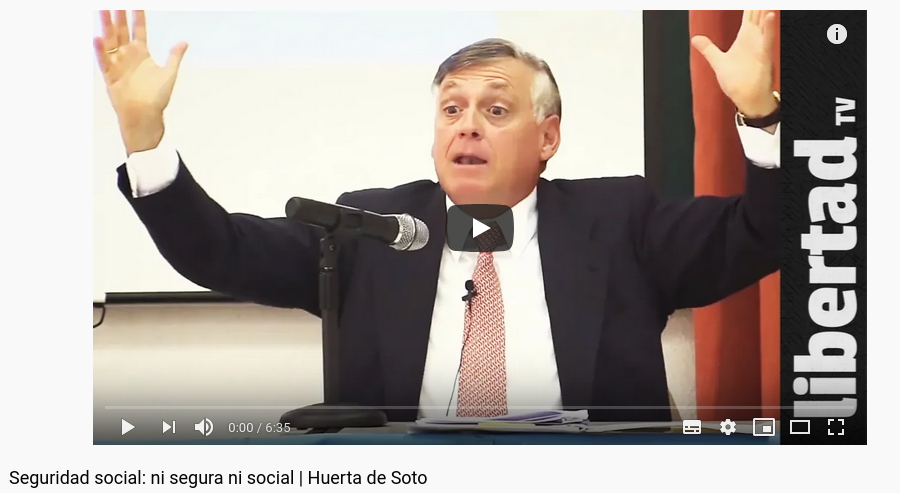
\includegraphics[width=0.75\textwidth]{figures/seguridad_social.png}
			\caption{\href{https://www.youtube.com/watch?v=NWA4nKAQjR4}{video de Huerta de Soto}}
		\end{figure}
		}
	\item Los paises se pueden endeudar, parece que infinitamente, por que hay mecanismos para <<imprimir dinero>> \textbf{INSERTAR REFERENCIA AQUI!} entre ellos destaca el banco central que es <<el diablo de la economia moderna>>
\end{itemize}

Mi humilde opinion es que estos principios inducen y animan al descontrol de las cuentas, pero como se puede \textbf{\textit{recibir sin dar nada a cambio}} en cierta medida, pues esto se convierte en un ciclo bastante toxico que algun dia explotara cuando la gente deje de confiar en elsistema y emigre hacia otras soluciones como el \textit{patron oro} \textbf{INSERTAR REFERENCIA AQUI!} o las \textit{soluciones descentralizadas como el \textbf{bitcoin}} \textbf{INSERTAR REFERENCIA AQUI!}\\

Es por esto, y por que yo con mis pocos anos de vida ya he vivido dos fuertes crisis, la de las hipotecas del 2008 \textbf{INSERTAR REFERENCIA AQUI!} y la de este presente ano, el coronavirus \textbf{INSERTAR REFERENCIA AQUI!} que yo abogo por una politica economica mas responsable desde el nivel mas bajo y fundamental de la cadena, el individual. A continuacion repaso muy brevemente dos puntos que me parecen fundamentales:

\subsection{Ahorra}

Ahorrar creo que es una de las cosas basicas de cualquier economia, ya estemos hablando a nivel individual, familiar, social o de estado, es basico ahorrar.\\

Por que, te puedes estar preguntando, pues muy sencillo, ahorrar te proporciona la capacidad para adquirir nuevos bienes y servicios. Cuanta mas capacidad de ahorro tengas mas podras comprar, haciendo un ciclo bastante rico propio de una economia prospera, pues si tu consigues dinero que puedes intercambiar por bienes y servicios, quienes los proporcionan tambien obtienen dinero y se va formando esta cadena.\\

\textbf{Haber ahorrado} tambien es fundamental en epocas de crisis como la que estamos viviendo ahora pues aunque quiebre la empresa en la que trabajas o seas despedido y no encuentres la oportunidad de un empleo podrias capear el temporal.\\

Por ultimo pero no menos importante, considero que uno de los mayores beneficios de ahorrar consiste en que cuando tenemos algo de capital y vemos una oportunidad de compra ya sea por ejemplo <<sobre ladrillo>>, en una empresa directamente o en el mercado de valores, podemos atacar sin dudar ni endeudarnos.

\subsection{Invierte}

Cuando hablo de invertir no me refiero unicamente a ir a comprar acciones de empresas en la bolsa de valores. \\

Yo considero una inversion todo lo que obtenemos o perseguimos, sin importar si es o no material, con la intencion de conseguir algun beneficio o rendimiento. Por ejemplo, podrias invertir en una dieta mas saludable o acorde a tus objetivos para acelerar el proceso de alcanzarlos, en este caso estarias comprando comida a cambio de mantener un cierto <<look>> o de alcanzar un fisico estetico o de simplemente estar mas sano. Das algo (dinero para comprar) y recibes algo a cambio (salud y estetica por ejemplo). Otro ejemplo seria comprar un buen ordenador para desarrollar tu trabajo en el caso de ser informatico por ejemplo. Como veremos en un posterior punto, yo no considero que tengas que gastarte una cantidad significativa de dinero para conseguir esto, hacieno un simil con la bolsa de valores seria como comprar acciones de una empresa cuando estan a 5\$, que otra persona las compre cuando estan a 90\$ y que actualmente se encuentren a 100\$. Con esto lo que intento decir es que tanto en la bolsa como al comprar un ordenador y todas las situaciones podemos hacer mejores o peores inversiones, el que se ha gastado solo 50\$ digamos por ejemplo, en un ordenador, pero es capaz de desarrollar el mismo trabajo que el que ha gastado 900\$ por ejemplo, suponiendo que el trabajo que realizan los dos es igual y les reportase 1000\$ de beneficio, habra hecho sin duda una inversion muchisimo mejor, mas inteligente.\\

Pero no nos equivoquemos, yo soy de los que piensa que algunas de las inversiones mas importantes que se hacen no se pagan con dinero, pero sin embargo reportaran enormes beneficios. Con esto me refiero a que la inversion mas importante que podemos hacer no tiene por que ser en nada material si no en nosotros mismos. A lo largo de estas paginas hemos hablado de como la independencia nos puede ayudar y aportar enormes beneficios, pero esto no se contruye con dinero, es un estado mental, un <<mindset>> que no podemos comprar. Asi, quiero decir que no podemos comprar valores. Por ejemplo, si tratasemos de pagar a alguien para que nos ayudase a hacer ejercicio pero nosotros por dentro no tuvieramos ambicion, determinacion, constancia y fuerza, no llegariamos muy lejos. 

Quizas te podrias estar preguntando que tiene todo esto que ver con la independencia, es muy sencillo. A la hora de hacer inversiones es normal en un primer momento tomar como referencia de buena inversion las inversiones que hace la mayoria de la gente, pero estas no tienen por que ser las mejores, esto es por lo que debemos ser independientes a la hora de invertir en lo que sea.\\

Eso si, para ser capaz de anticiparse o de poder sustentar opiniones distintas al resto y por tanto poder realizar inversiones distintas hay que aprender mucho sobre los temas que nos interesan y en la mayoria de las ocasiones esto es un trabajo duro que no veremos recompensado inmediatamente si no cuando realicemos la inversion y conozcamos el resultado sabiendo si lo hemos hecho mejor o peor que el que no se informo sobre el tema.\\

Aunque creo que puedo adelantar sin problema que el que conoce un tema a fondo es capaz de realizar mejores inversiones que los demas, animo a la gente a que prueben esta metodologia antes de lanzarse a comprar un producto, adquirir un servicio o invertir tiempo en una actividad. En mi experiencia es seguro tambien que cuanto mas vayas profundizando, mejores inversiones vas a ir realizando, pues pensar que la primera inversion que realices sera increible es algo que creo que dista de la realidad. Esto es como todo, se aprende haciendo.

\section{Independencia en la informatica}

En esta parte vamos a hablar de que considero yo que es la independencia en informatica y como alcanzarla o perseguirla. Para esto dividire el apartado en dos, constara de una primera parte en la que hablaremos brevemente sobre el hardware, una segunda sobre el software y al final dare una nota.

\subsection{ Hardware }

Cuando hablamos de independencia en el hardware, estoy haciendo referencia a varias caracteristicas que se juntan para ofrecer lo mejor. 

La primera de estas partes es la habilidad que tenemos para saber lo que "gastan", o los recursos que consumen las aplicaciones que utilizamos, esto es fundamental en un primer momento a la hora de elegir un hardware, pues si las aplicaciones que utilizamos son las de uso comun general, por ejemplo navegadores de internet y aplicaciones de ofimatica, no parece tener mucho sentido ir a por una cpu de gama alta o muy alta. El sistema funcionara a la perfeccion, pero estaremos desperdiciando ese hardware que probablemente "pida" un uso mas intensivo. Es como comprarse un coche de 100.000\$ para llevar a los chicos al colegio...Nos resultara mucho mas costoso que si elegimos un coche normalito que sea fiable incluso de segunda mano por lo que obtendremos una rebaja sustancial, asi podriamos \textbf{ completar la misma tarea con poca diferencia en rendimiento por una fraccion del precio. } De la misma forma, en vez de comprar los componentes mas potentes para nuestro ordenador, sabiendo que probablemente no les vayamos a dar un uso intensivo ni la mitad del tiempo, te recomiendo buscar componentes que ofrezcan menor rendimiento a mucho menor precio, incluso informarte y rebuscar entre componentes algo antiguos, estoy seguro de que te podria llegar a sorprender lo barato que puede resultar un ordenador que haga lo que tu necesites.

Otro aspecto muy importante es la capacidad que tiene el hardware para ser \textbf{ extensible }, esto es, que si comenzamos en el mundo de la informatica con un procesador de gama baja, pongamos un intel core 2 duo por ejemplo, pero pasado un tiempo nos damos cuenta de que necesitamos algo mas potente por que las tareas que realizamos son demasiado pesadas, tener la capacidad de poder cambiar ese componente con facilidad. Esto se hace especialmente dificil en el mundo de los portatiles modernos, que son casi "de usar y tirar" y si quieres uno que te dure mucho lo que tienes que hacer es gastar mas. Yo estoy en contra de esto en la mayoria de los casos, hay marcas que hacen portatiles que son muy faciles de modificar, no hace falta ni si quiera llevarlo a un tecnico. Por ejemplo lenovo con sus thinkpad, especialmente los antiguos incluso los de IBM. En ordenadores de sobremesa es relativamente mas sencillo hacer algun cambio de componentes si elegimos una configuracion inicial interesante y apta para ello. Esto por ejemplo hablando de la cpu se logra eligiendo una placa base cuyo socket soporte diferentes gamas de la misma cpu, por ejemplo un i3, i5 e i7. 

Estoy hablando bastante de las cpus, pero otra caracteristica importante a la hora de plantearnos cambiar algun componente del ordenador o incluso cambiar de ordenador es reconocer que va mal o "lento". Si por ejemplo lo que pasa es que cuando vemos peliculas estas tardan mucho en renderizar o incluso no las podemos ver a la resolucion que quisieramos y ademas todo el sistema es muy lento y encima produce mucho calor o ruido, es decir, si todas las partes del ordenador nos dan problemas es buena idea quizas pensar en cambiar de software y en ultima instancia de ordenador. Por otro lado si lo unico que pasa es que el sistema se siente lento, no debemos pensar de primeras en tirarlo y comprar otro, es buena idea por ejemplo investigar el tipo de disco que tiene, ya que si es uno mecanico puede que esa sea la fuente de los problemas, y es mucho mas barato comprar una unidad de estado solido (SSD) y sustituirlo en el equipo que comprar un equipo nuevo. 

Si no estas teniendo una buena experiencia con tu ordenador o crees que no te esta ofreciendo todo lo que necesitas te recomiendo hacer varias consideraciones como investigar la posibilidad de instalar otro sistema operativo, ya que probablemente tengas windows y esto sea la mayor fuente de problemas. Asi podrias investigar algo como instalar un sistema operativo Linux, o investigar los componentes hardware de tu equipo para ver si logras identificar algun cuello de botella importante y ver si es posible cambiar esa parte.

Como nota final he de decir que a mi personalmente me gusta comprar hardware de segunda mano, considero que es un buen mercado por que hay gente que consume y tira los equipos sin saber muy bien que a lo mejor alguna de las piezas de las que va a deshacerse es de mucha calidad y aunque sea antigua puede durar mucho tiempo mas con un mantenimiento adecuado. Yo me monte un sistema asi, con una placa P6T deluxe V2 que va de lujo y que tiene mucha mucha calidad, la compre a una fraccion del precio de lo que cuesta, compre una cpu intel i7 (era la unica opcion que conocia en el momento, ahora he aprendido que se pueden instalar algunos intel Xeon) 4gb de ram y una unidad de estado solido. Esto y algunas piezas mas que hacen falta me costo menos de 200\$ y es un sistema que lleva ya conmigo 2 anos y que durara bastante mas. En cuanto a portatiles, estoy orgullosos de decir que estoy realizando todo este trabajo desde un IBM/Lenovo Thinkpad T60, un portatil de 2006, que funciona a la perfeccion. Le instale algo mas de memoria ram y una unidad de estado solido y va como un tiro. Se le puede tambien cambiar la cpu lo cual hare e incluso la pantalla...La mejor parte es que me costo 50\$ !

\subsection{ Software }

Cuando me monte mi primer ordenador de segunda mano me di cuenta de que Windows costaba mucho dinero, y aunque podia hacer algun apano para que me costase menos, decidi irme por un sistema linux, Ubuntu, que funcionaba bastante mejor. A medida que me fui adentrando en el mundillo me di cuenta de que se pueden conseguir setups software que usan muy poquitos recursos hardware y desde entonces es una de mis metas conseguir un setup hardware + software que sirva para realizar tareas cotidianas sin comproisos. Algunos ejemplos geniales de esto son los SOC \textbf{INSEERTAR REFERNCIA} como las Raspberry Pi (en concreto la version 4) \textbf{INSERTAR IMAGEN}, que son un dispostivo que ofrecen un ordenador con buen rendimiento, mas del que mucha gente necesita, por menos de 100\$.

Centrandonos ahora en el ambito del software, pronto descubri que algunas aplicaciones graficas, o GUI, son en bastantes casos extremadamente ineficientes, pues lo unico que hacen es poner de forma grafica con botones y menus (esto gasta muchos recursos hardware) lo que es o podria ser realmente una aplicacion de consola con las mismas opciones y menus y consumiendo muchos menos recursos...

Como ejemplo pongamos los IDE, como Eclipse \textbf{INSERTAR REFERENCIA} y eso que este no es el peor ejemplo que se me ocurre pues al menos es de codigo abierto, pero sirve para ejemplificar lo que quiero demostrar. Esta aplicacion nos proporciona un entorno grafico con muchos paneles y botones ( que son muy liosos, no es facil encontrar las opciones... ) todo ello para ser capaces de escribir un texto (codigo) en un panel y poder darle a un boton verde que compila el codigo y lanza la aplicacion que estemos construyendo. En la facultad recuerdo que paso que una clase entera de alumnos suspendio un examen por que el entorno estaba mal configurado, y es que la configuracion de estos entornos puede llegar a ser infernal. Yo opto por tener mas control sobre lo que estoy haciendo y simplificar los procesos, independizando cada uno de los pasos que hay que dar pero consiguiendo mucha mas velocidad y mejor rendimiento... Pongo un ejemplo de como estoy haciendo este poryecto o como hago otros que requieren codigo:

\begin{itemize}

\item Edito un archivo de texto en un editor como vim, pero hay otros e incluso puede ser uno grafico que sea muy ligero, yo usaba gedit antes cuando usaba gnome. 

\item Compilo ese archivo con el compilador que yo quiero y que se que va a funcionar y las opciones o flags que me convienen.

\item Lanzo la aplicacion , lo cual es trivial pues en el paso anterior se me ha generado un ejecuable.

\item Por ultimo repito todos los pasos anteriores hasta que tengo el producto final. Si hay que debugear la cosa se puede poner un poco mas compleja, pero una vez aprendes a usar minimamente gdb y a debugear sobre el codigo en la ejecucion del programa, todo se vuelve mas sencillo.

\end{itemize}

Y algunos direis, vale, esto puede estar bien, pero es mucho mas lento y tengo que hacer mas trabajo que si estoy en un entorno y le doy a un boton. Aqui entra la magia de este software, pues al ser muy extensible puedo configurar de forma sencilla y segura un boton en el teclado por el cual se pasa la ruta del archivo que estoy editando a un script que se llama compilar y que tiene una distincion de casos segun la extension del archivo y ahi especifico los compiladores que quiero segun el caso. Asi:

\begin{itemize}

\item
logro tener mucho control, por que yo elijo cada una de las partes segun mis preferencias
\item fiabilidad, por que los mecanismos usados son practicamente atomicos, hay nula o poca configuracion de por medio
\item velocidad, pues una vez controlo los dos puntos anteriores puedo optimizar el proceso automatizandolo a mi gusto.

\end{itemize}

Esta es la base de como uso yo un ordenador, no me conformo con lo que viene dado en un cierto sistema operativo, como por ejemplo Ubuntu. Me gusta toquetear e instalar como interfaz grafica un Tiling window manager \textbf{INSERTAR REFERENCIA AQUI!} como xmonad o dwm \textbf{INSERTAR REFERNCIA AQUI!} y construir "mi propio sistema operativo", esto es, elegir las aplicaciones que ami me gustan, configurarlas y optimizarlas segun mis necesidades. Asi puedo elegir como editor neovim \textbf{INSERTAR REFERENCIA}, como navegador de internet Lynx \textbf{INSERTAR REFERENCIA} , w3m \textbf{INSERTAR REFERENCIA} , surf \textbf{INSERTAR REFERENCIA} o brave \textbf{INSERTAR REFERENCIA}. Puedo automatizar tareas o construir mis propias aplicaciones como mi navegador de ficheros \textbf{INSERTAR REFERENCIA} sobre otras aplicaciones super extensibles como dmenu \textbf{INSERTAR REFERENCIA}, etc etc...  

Asi, te animo a identificar software en tu sistema que es ineficiente e investigar cuales son las alternativas y si hay alguna que resulte mas interesante. Un ejemplo bueno para el publico general son los editores de PDF, los de adobe o similares pueden resultar en desesperanza por lo que tardan en cargar o lo que pueden llegar a costar, sin embargo hay aplicaciones como Xournalpp que te podrian sorprender.

Por ultimo en este apartado me gustaria hacer una mencion especial a los programas online o en la nube que ofrecen servicios muy interesantes y no requieren de instalar. Mi opinion personal es que no los uses a menos de que seas consciente que es probable que algunos de esos programas esten obteniendo redito economico, vendiendo tu informacion por ejemplo, a cambio de que los uses...Sin embargo esto lo considero buena opcion si la nube que usas es tuya, por ejemplo puedes hacer una instalacion de Nextcloud \textbf{INSERTAR REFERENCIA} que es fantastico para esta tarea, en un servidor fisico en tu casa o uno alquilado en un proveedor como DigialOcean \textbf{INSERTAR REFERENCIA} y asi asegurar lo maximo posible que tu eres el unico "beneficiario" del uso de ese tipo de programas, pero la idea de poder usar programas que serian muy pesados para nuestro dispositivo, alojandolos en servidores mas potentes me parece una idea genial.


\chapter{Algunas notas finales}

\listoffigures
\bibliographystyle{unsrt}
\bibliography{citations/citations}
}
\end{document}

